\documentclass[tikz, border=10pt]{standalone}
\usetikzlibrary{shapes.geometric, arrows.meta, positioning, calc, matrix, backgrounds, shadows}

\begin{document}
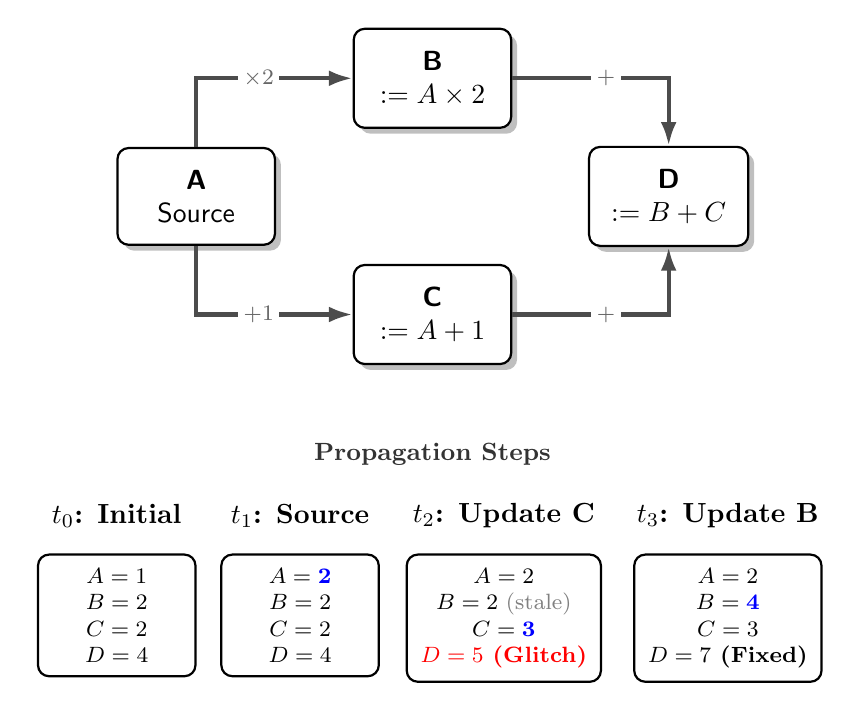
\begin{tikzpicture}[
    font=\sffamily,
    thick,
    % --- Main Component Style ---
    component/.style={
        draw=black, 
        fill=white, 
        thick, 
        rounded corners,
        align=center,
        inner sep=8pt,
        drop shadow,
        minimum width=2cm,
        minimum height=1.2cm
    },
    % --- Connecting Arrows ---
    dep arrow/.style={
        -{Latex[length=3mm, width=2mm]}, 
        line width=1.5pt,
        color=gray!60!black
    },
    % --- Edge Labels ---
    edge label/.style={
        font=\footnotesize\bfseries,
        midway,
        fill=white,
        inner sep=2pt,
        text=gray!80!black
    },
    % --- Text Labels ---
    label text/.style={
        font=\bfseries\small,
        color=gray!40!black
    },
    % --- Matrix/Timeline Styles ---
    time header/.style={
        font=\bfseries,
        text=black,
        align=center,
        anchor=south
    },
    time cell/.style={
        draw=black, 
        fill=white, 
        rounded corners, 
        align=center,
        font=\footnotesize,
        inner sep=5pt,
        minimum width=2cm
    }
]

    % =========================================
    % 1. SYMMETRIC DIAMOND GRAPH
    % =========================================

    % Node A (Source) - Left
    \node[component] (nodeA) at (0,0) {
        \textbf{A} \\ Source
    };

    % Node B (Top) - Middle
    % Aligned vertically relative to center, horizontally offset
    \node[component] (nodeB) at (3, 1.5) {
        \textbf{B} \\ $:= A \times 2$
    };

    % Node C (Bottom) - Middle
    % Symmetric to B
    \node[component] (nodeC) at (3, -1.5) {
        \textbf{C} \\ $:= A + 1$
    };

    % Node D (Sink) - Right
    % Aligned horizontally with A (y=0), offset by 6cm
    \node[component] (nodeD) at (6, 0) {
        \textbf{D} \\ $:= B + C$
    };

    % Dependencies (Edges)
    \draw[dep arrow] (nodeA) |- (nodeB) node[edge label, pos=0.7] {$\times 2$};
    \draw[dep arrow] (nodeA) |- (nodeC) node[edge label, pos=0.7] {$+ 1$};
    
    \draw[dep arrow] (nodeB) -| (nodeD) node[edge label, pos=0.3] {$+$};
    \draw[dep arrow] (nodeC) -| (nodeD) node[edge label, pos=0.3] {$+$};

    % =========================================
    % 2. STATE EVOLUTION TABLE (The Glitch)
    % =========================================
    
    % Using standard \matrix (not matrix of nodes) for safety with multi-line text
    \matrix[
        row sep=0.2cm,
        column sep=0.3cm,
        below=1.5cm of nodeC.south, % Anchor below the graph
        anchor=north
    ] (timeline) {
        % Header Row
        \node[time header] {$t_0$: Initial}; & 
        \node[time header] {$t_1$: Source}; & 
        \node[time header] {$t_2$: Update C}; & 
        \node[time header] {$t_3$: Update B}; \\
        
        % Data Row
        \node[time cell] {
            $A=1$\\
            $B=2$\\
            $C=2$\\ 
            \textbf{$D=4$}
        }; & 
        \node[time cell] {
            $A=\textbf{\textcolor{blue}{2}}$\\
            $B=2$\\
            $C=2$\\ 
            $D=4$
        }; & 
        \node[time cell] {
            $A=2$\\
            $B=2$ \textcolor{gray}{(stale)}\\
            $C=\textbf{\textcolor{blue}{3}}$\\ 
            \textbf{\textcolor{red}{$D=5$ (Glitch)}}
        }; & 
        \node[time cell] {
            $A=2$\\
            $B=\textbf{\textcolor{blue}{4}}$\\
            $C=3$\\ 
            \textbf{$D=7$ (Fixed)}
        }; \\
    };
    
    % Label for the table
    \node[label text, above=0.1cm of timeline.north] {Propagation Steps};

\end{tikzpicture}
\end{document}
